\documentclass[11pt,a4paper]{article}
\usepackage[margin=25mm,headheight=15pt]{geometry}
\usepackage[T1]{fontenc}
\usepackage[utf8]{inputenc}
\usepackage{lmodern}
\usepackage{microtype}
\usepackage{graphicx}
\usepackage{booktabs}
\usepackage{array}
\usepackage{longtable}
\usepackage{fancyhdr}
\usepackage{hyperref}
\usepackage{xcolor}
\usepackage{setspace}
\usepackage{caption}
\usepackage{enumitem}
\usepackage{amsmath}
\usepackage{url}
\definecolor{ink}{HTML}{183549}
\definecolor{muted}{HTML}{566573}
\hypersetup{colorlinks=true,linkcolor=ink,citecolor=ink,urlcolor=ink,pdftitle={Genomic Investigation of MRSA Virulence and Antimicrobial Resistance},pdfauthor={Tharuniya Anpalakan}}
\captionsetup{font=small,labelfont=bf,skip=6pt}
\setstretch{1.12}
\setlength{\parindent}{0pt}
\setlength{\parskip}{0.56em}
\setlist[itemize]{leftmargin=1.5em,itemsep=0.15em,topsep=0.2em}
\pagestyle{fancy}
\fancyhf{}
\fancyhead[L]{\footnotesize\color{muted}MRSA GENOMICS / RESEARCH REPORT}
\fancyhead[R]{\footnotesize\color{muted}THARUNIYA ANPALAKAN}
\fancyfoot[C]{\footnotesize\thepage}
\renewcommand{\headrulewidth}{0.25pt}
\setcounter{secnumdepth}{2}
\begin{document}
\hypersetup{pageanchor=false}

\begin{titlepage}
\thispagestyle{empty}
\vspace*{22mm}
{\color{ink}\rule{\textwidth}{1.1pt}}\\[8mm]
{\small\bfseries\color{muted}COMPUTATIONAL GENOMICS / TECHNICAL RESEARCH REPORT}\par
\vspace{18mm}
{\Huge\bfseries\color{ink}Genomic Investigation of\\[2mm]MRSA Virulence and\\[2mm]Antimicrobial Resistance\par}
\vspace{7mm}
{\large Comparative analysis framework for public \textit{Staphylococcus aureus} assemblies\par}
\vspace{17mm}
{\large Tharuniya Anpalakan\par}
{\small Project Author\par}
\vspace{5mm}
\vfill
\begin{minipage}{0.84\textwidth}
\color{muted}\small
\textbf{Study status.} Four versioned public assemblies have been acquired and assessed with an exploratory FASTA quality-control screen. Resistance and virulence gene calling, molecular typing, and genotype--phenotype comparisons await the specified external tools and verified metadata. This document reports the completed assembly analysis and defines the remaining computational work without treating planned analyses as findings.
\end{minipage}
\vspace{12mm}\\
{\color{ink}\rule{\textwidth}{0.6pt}}
\end{titlepage}
\hypersetup{pageanchor=true}

\begin{abstract}
\noindent\textbf{Background.} Genome sequencing can identify known resistance and virulence determinants in \textit{Staphylococcus aureus}, provided that assemblies, reference databases, and isolate metadata are adequately documented. \textbf{Objective.} This study establishes a reproducible workflow for a small collection of public reference assemblies and evaluates the assembly data available before molecular screening. \textbf{Methods.} Four distinct, versioned NCBI RefSeq assemblies were selected as a technical demonstration cohort. Downloaded FASTA files were checked for valid sequence identifiers and characters, and assembly length, GC content, N50, sequence-record count, and ambiguous-base fraction were calculated. A predefined exploratory screen was applied. \textbf{Results.} All four files passed this screen. Assembly lengths ranged from 2,820,462 to 2,917,469 bp; sequence-record counts ranged from one to four. \textbf{Interpretation.} These are assembly-level observations, not evidence of completeness, antimicrobial susceptibility, toxin expression, or clinical phenotype. AMRFinderPlus screening and typing remain unexecuted in the present environment. The cohort cannot support population prevalence or acquisition-setting comparisons.
\end{abstract}

\section{Introduction}
\textit{Staphylococcus aureus} is a Gram-positive coccus that colonizes the skin and mucosa of humans and can cause skin and soft-tissue infection, bacteremia, pneumonia, endocarditis, and other invasive disease. Colonization, host susceptibility, local tissue conditions, and strain-specific traits all contribute to the transition from carriage to infection \cite{Tong2015,Foster2004}. Methicillin-resistant \textit{S. aureus} (MRSA) is of particular interest because resistance to many beta-lactams can constrain treatment and because successful lineages circulate through both community and healthcare settings. Epidemiological labels describe where and how infection was acquired; they cannot be assigned solely from a genomic signature.

This project asks: \emph{What antimicrobial resistance and virulence determinants can be identified in a reproducibly selected collection of publicly available \textit{S. aureus} genomes, and how do their distributions vary across the available isolate metadata?} The question is conditional. A sequence-based screen can address gene content only when the caller, reference database, and target coverage are validated. A comparison between isolate groups requires authentic group metadata, and a genotype--phenotype comparison additionally requires susceptibility measurements. The current report therefore presents the completed acquisition and assembly QC, then specifies how the later stages should be carried out.

\section{Biological and genomic context}
\subsection{Methicillin resistance and SCCmec}
The most familiar MRSA mechanism is acquisition of \textit{mecA}, which encodes the alternative penicillin-binding protein PBP2a. Because PBP2a has reduced affinity for many beta-lactam agents, cross-linking of peptidoglycan can continue when native penicillin-binding proteins are inhibited. PBP2a is not simply a point-mutated version of a native protein: it is the product of an acquired determinant. A divergent homologue, now termed \textit{mecC}, has also been documented in human and animal-associated \textit{S. aureus} \cite{Foster2004,GarciaAlvarez2011}.

Methicillin-resistance determinants are commonly embedded within staphylococcal cassette chromosome \textit{mec} (SCCmec), a mobile element with a \textit{mec} gene complex, cassette chromosome recombinase genes, and variable joining regions. SCCmec type is defined by the element's architecture. A \textit{mecA} hit alone cannot identify SCCmec IV or any other type \cite{IWGSCC2009}. The historical association of some community-associated MRSA lineages with compact SCCmec IV elements is useful background, but it is neither an exclusive molecular rule nor a substitute for patient-level epidemiological information \cite{Baba2002,Diep2006}.

\subsection{Tetracycline resistance}
Tetracyclines act at the bacterial 30S ribosomal subunit and interfere with aminoacyl-tRNA entry during translation. Acquired resistance can arise through efflux, including Tet(K) and Tet(L), or ribosomal protection, including Tet(M) and Tet(O) \cite{Chukwudi2016}. The presence of a named determinant does not, by itself, specify a susceptibility category for every tetracycline-class compound; expression, allele, drug, breakpoint, and laboratory method matter. Conversely, a negative sequence call cannot establish susceptibility, especially when assembly quality, gene divergence, or database coverage is uncertain. In this study no isolate-level tetracycline phenotype has been verified.

\subsection{Virulence markers and PVL}
Panton--Valentine leukocidin (PVL) is a bicomponent toxin encoded by \textit{lukS-PV} and \textit{lukF-PV}. The protein subunits act together to form pores in susceptible host leukocytes; receptor studies implicate human C5a receptors in cell targeting \cite{Aman2014,Spaan2013}. Hemolysins and adhesion-associated factors, including alpha-toxin and clumping or fibronectin-binding proteins, contribute to the wider virulence repertoire. Genomic detection is evidence of a sequence related to a known determinant, not direct evidence of transcription, protein abundance, toxin activity, host response, or disease severity.

PVL has been associated with particular skin and soft-tissue presentations, but its clinical contribution differs by syndrome and study design. A systematic review found that broad claims about PVL as an independent determinant of severe disease are not warranted \cite{Shallcross2013}. PVL status is therefore treated as a potential genomic observation to be assessed after validated screening, not as a defining feature of community acquisition.

\section{Study design and data provenance}
\subsection{Selection rule}
Four distinct, named, complete NCBI RefSeq assemblies were fixed before QC: N315, MW2, MRSA252, and USA300\_FPR3757. Their original sequencing publications provide historical context \cite{Kuroda2001,Baba2002,Holden2004,Diep2006}. This is a compact, deliberately selected reference-genome demonstration rather than a random or representative sample of circulating MRSA. One versioned assembly per named strain was retained. No selection was made on the basis of the QC outcomes reported below.

\begin{table}[htbp]
\centering\small
\caption{Public genome cohort. BioSample accessions and genome URLs are recorded in the repository manifest. Empty clinical fields were not imputed.}
\begin{tabular}{@{}lllp{45mm}@{}}\toprule
Strain & RefSeq assembly & BioSample & Verified contextual note\\\midrule
N315 & GCF\_000009645.1 & SAMD00061099 & Published reference strain\\
MW2 & GCF\_000011265.1 & SAMD00061104 & Published reference strain\\
MRSA252 & GCF\_000011505.1 & SAMEA1705935 & Hospital-associated description in BioProject\\
USA300\_FPR3757 & GCF\_000013465.1 & SAMN02604150 & USA300 lineage; acquisition setting of specimen unverified\\\bottomrule
\end{tabular}
\label{tab:cohort}
\end{table}

The manifest preserves source URLs, accession versions, assembly level, source database, metadata availability, and a selection rationale. Collection year, country, isolation source, sequencing platform, and antimicrobial susceptibility data remain blank where no reliable isolate-level record was established. The genomes were obtained on 17 October 2026. The compressed files are excluded from Git; observed SHA-256 digests are retained in the tracked metadata directory so a future download can be checked. Versioned accession identifiers and source links permit independent retrieval \cite{NCBI_Datasets}.

\subsection{Scope of comparison}
The four assemblies represent different named reference strains and historical studies. That diversity is useful for exercising a pipeline, but the cohort is too small and purposively assembled for population prevalence estimates or significance testing. The available metadata do not establish a consistent community-versus-healthcare classification for each sequenced specimen. The report consequently makes no such group comparison and no inference about transmission.

\section{Computational methods}
\subsection{Acquisition and FASTA validation}
The acquisition module downloads each exact HTTPS `genomic.fna.gz' file listed in the manifest. It rejects malformed or duplicate RefSeq accessions, checks the expected NCBI URL prefix, verifies gzip integrity and FASTA start, and compares downloaded compressed-file hashes with the tracked SHA-256 values. The QC module streams each sequence record and rejects empty files, duplicate or missing record identifiers, and characters outside A, C, G, T, and N. These checks detect obvious file and formatting problems; they cannot establish read-level quality or assembly completeness.

\subsection{Assembly metrics and decision rule}
Total length is the sum of all FASTA-record lengths, including plasmid records where present. GC fraction is the number of G and C bases divided by that total; ambiguous fraction is the number of N bases divided by the same total. N50 is the length of the sequence record at which the cumulative length of records sorted from longest to shortest reaches at least half of the total assembly length. The quality screen flags an assembly for review if its total length lies outside 2.5--3.2 Mbp, if it has more than 20 records, or if more than 1\% of bases are N. These pragmatic bounds were chosen for this complete-reference demonstration and are not a universal acceptance criterion for \textit{S. aureus}. No independent completeness or contamination estimator was run.

\subsection{Determinant screening and typing: specified, not executed}
The repository includes an AMRFinderPlus wrapper for consistent assembly-level screening. Its specified invocation uses nucleotide assemblies, the \textit{S. aureus} organism option, and the `--plus' option for curated non-AMR categories. The wrapper preserves the native tab-separated output, extracts positive AMR calls, and records software/database versions and reported identity and coverage values. A separate parser extracts explicitly labelled virulence calls. These methods follow the curated-reference approach described for AMRFinder and AMRFinderPlus \cite{Feldgarden2019,Feldgarden2021,NCBI_AMRFinderPlus}. The executable and database were not available in the present Windows environment, so no gene calls were made.

Before interpreting a non-call for \textit{mecA}, \textit{mecC}, a tet-family member, or either PVL component, the reference database must be audited for that target and the native output checked for partial or ambiguous alignments. A positive hit should be considered with its identity, reference coverage, method and genomic context. Sequence typing requires a validated multilocus-sequence-typing implementation and allele database \cite{Enright2000}; SCCmec assignment requires cassette-level evidence \cite{IWGSCC2009}. Neither typing analysis was performed here.

\subsection{Descriptive analysis}
The completed statistics are the number of selected assemblies, the number passing exploratory QC, and observed metric ranges. A Wilson score interval is implemented in the code for future fully assessed binary outcomes \cite{Wilson1927}, but no marker interval is reported because no complete, validated marker screen exists. Gene-call status remains `not assessed' rather than being silently recoded as absence. No hypothesis test was attempted on this four-genome convenience cohort.

\section{Results: completed assembly quality control}
All four versioned assemblies were retrieved and parsed. Each passed the predefined size, sequence-record-count, and ambiguous-base screen (Table~\ref{tab:qc}). N315 and USA300\_FPR3757 contain more than one FASTA record; the total lengths therefore include all supplied sequence records, not solely the main chromosome. The complete numerical output is available as a machine-readable CSV in the repository.

\begin{table}[htbp]
\centering\small
\caption{Observed FASTA assembly metrics. GC and N percentages use total assembly length as denominator. `Pass' applies only to the predefined exploratory screen.}
\begin{tabular}{@{}lrrrrrl@{}}\toprule
Strain & Length (bp) & GC (\%) & Records & N50 (bp) & N (\%) & Screen\\\midrule
N315 & 2,839,469 & 32.808 & 2 & 2,814,816 & 0.000 & Pass\\
MW2 & 2,820,462 & 32.830 & 1 & 2,820,462 & 0.000 & Pass\\
MRSA252 & 2,902,619 & 32.807 & 1 & 2,902,619 & 0.000 & Pass\\
USA300\_FPR3757 & 2,917,469 & 32.691 & 4 & 2,872,769 & 0.000 & Pass\\\bottomrule
\end{tabular}
\label{tab:qc}
\end{table}

\begin{figure}[htbp]
\centering
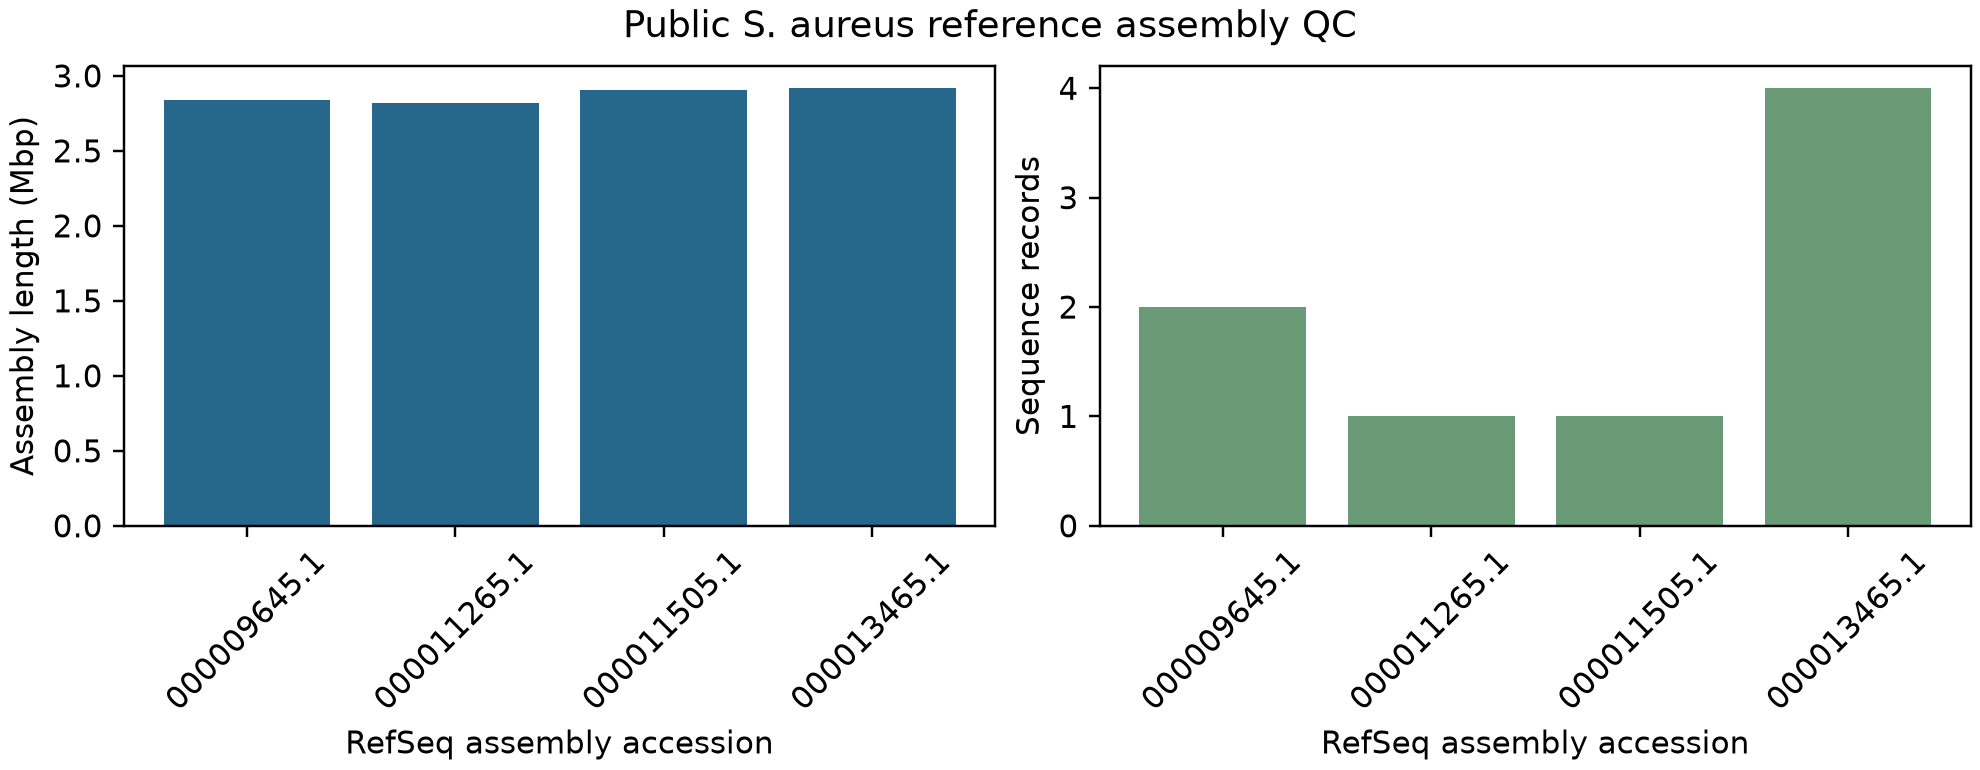
\includegraphics[width=0.92\linewidth]{../figures/genome_qc.png}
\caption{Assembly length and FASTA-record count for the four downloaded RefSeq assemblies. The figure is generated directly from \texttt{results/genome\_qc.csv}; it does not display resistance or virulence findings.}
\label{fig:qc}
\end{figure}

The observed length range is 2,820,462--2,917,469 bp, and the sequence-record count ranges from one to four. All downloaded sequences contain zero N bases under the implemented counting rule. These observations neither validate species identity nor rule out contamination, structural errors, or missing genes. There are no AMR, virulence, MLST, SCCmec, or susceptibility results to report.

\section{Discussion}
The acquisition and QC stages establish a traceable starting point for comparative genomics. Exact accession versions, BioSample identifiers, URLs, checksums, and the screening rule make the completed stage inspectable. At the same time, this cohort is a poor basis for biological frequency estimates: it is small, historically selected, and drawn from distinct studies and lineages. The all-pass QC result indicates only that the downloaded assemblies meet the stated elementary thresholds, not that all biologically relevant loci are complete and accurately assembled.

Future AMRFinderPlus output could support statements such as `a reference sequence assigned to a named determinant was detected under a documented database version and method'. It would not alone prove a resistant phenotype or a virulence effect. In particular, PVL gene detection would not establish active toxin production, and \textit{mecA} detection would not establish an SCCmec type. Genotype--phenotype evaluation requires authenticated antimicrobial susceptibility records, drug-specific interpretive criteria, and attention to discordant calls. The present manifest contains no such phenotype data.

The historic source coursework described a patient-specific MRSA scenario but supplied no isolate accession, AST measurements, or sequence data for that patient. Those statements were therefore treated as background claims requiring review rather than transferred into this study's results. Original source figures were retained privately because reuse rights were not verified. No bacterial culture, sequencing, clinical testing, or wet-laboratory work is attributed to the computational project author.

\section{Limitations and next analysis steps}
\begin{itemize}
\item The four reference assemblies are a convenience cohort; inference to contemporary MRSA populations is inappropriate.
\item The QC stage has not used raw reads or a validated completeness/contamination estimator.
\item AMRFinderPlus and its database have not run on these assemblies. The code is ready for execution in a compatible environment, followed by native-output review and database coverage checks.
\item MLST and SCCmec typing need dedicated tools and manual evaluation of confidence, especially if cassette structure is fragmented.
\item No consistent collection, acquisition-setting, or authentic susceptibility metadata were verified; those comparisons must wait for suitable records.
\item A phylogeny was omitted because homologous alignment, recombination assessment, and an appropriate sampling design have not been completed.
\end{itemize}

\section{Conclusion}
Four public, versioned \textit{S. aureus} assemblies were acquired and passed a documented exploratory FASTA QC screen. The principal research questions about resistance and virulence determinants remain open until validated screening is executed and its reference coverage reviewed. The resulting repository is a reproducible technical foundation for analysis, not a completed molecular survey or clinical diagnostic report.

\section*{Reproducibility statement}
The repository contains the exact manifest, tracked download checksums, source code, tests, notebook views, and figure-generation code. On a fresh clone, install the documented Python environment and run the acquisition, QC, and visualization modules from the repository root. This PDF was compiled from the LaTeX source in the \texttt{reports} directory with BibTeX entries in \texttt{references}. Run \texttt{python reports/build\_latex.py} to rebuild it. The completed QC used Python 3.14.2, pandas 3.0.6, and Matplotlib 3.11.2; AMRFinderPlus was not installed or run.

\bibliographystyle{unsrt}
\bibliography{../references/bibliography}
\end{document}
